\documentclass[aspectratio=169,usenames,dvipsnames]{beamer}
\mode<presentation>
\usefonttheme{professionalfonts}

\usetheme[height=0pt]{Rochester}
\useinnertheme{circles}
%\setbeamertemplate{blocks}[rounded][shadow=false]
\setbeamercolor{math text}{fg=RedOrange}
\setbeamercolor{frametitle}{fg=Plum}
\setbeamercolor{framesubtitle}{fg=MidnightBlue}
\setbeamercolor{emph}{fg=MidnightBlue}
\setbeamercolor{block title}{bg=Plum,fg=white}
\setbeamercolor{footlinecolor}{fg=Plum,bg=white}
\renewcommand<>{\emph}[1]{%
  {\usebeamercolor[fg]{emph}\only#2{\itshape}#1}% chktex 6
}
\setbeamertemplate{frametitle}
{%
\begin{centering}
\insertframetitle\par
\insertframesubtitle\par
\end{centering}
}
\beamertemplatenavigationsymbolsempty%
% 20180504: For reasons unknown, the following line stopped working, so we have
% to use the one after it.
%\setbeamertemplate{footline}[frame number]
\setbeamertemplate{footline}{%
  \begin{beamercolorbox}[sep=.5em,wd=\paperwidth]{footlinecolor}
    \hfill
    \scriptsize{\insertframenumber}
  \end{beamercolorbox}%
}
\addtobeamertemplate{block
begin}{\setlength\abovedisplayskip{0pt}\setlength\belowdisplayskip{0pt}\setlength\abovedisplayshortskip{0pt}\setlength\belowdisplayshortskip{0pt}}

\newcommand{\plum}{\color{Plum}}
\newcommand{\purple}{\color{purple}}
\newcommand{\black}{\color{black}}
\newcommand{\green}{\color{ForestGreen}}
\newcommand{\red}{\color{red}}
\newcommand{\blue}{\color{MidnightBlue}}
\newcommand{\pinegreen}{\color{PineGreen}}
\newcommand{\bittersweet}{\color{Bittersweet}}
\newcommand{\orange}{\color{RedOrange}}

%! TEX root = diffusr.tex
% Keep the list in alphabetical order, unless is really helpful to break it =)
\usepackage{accents} % to use custom accents
\usepackage[ruled,vlined,linesnumbered]{algorithm2e}
\usepackage{cleveref}
\crefname{algorithm}{Alg.}{Algs.}
\Crefname{algorithm}{Algorithm}{Algorithms}
\crefname{appendix}{App.}{App.}
\Crefname{appendix}{Appendix}{Appendices}
\crefname{corollary}{Corol.}{Corolls.}
\Crefname{corollary}{Corollary}{Corollaries}
\crefname{conjecture}{Conjecture}{Conjectures}
\Crefname{conjecture}{Conjecture}{Conjectures}
\crefformat{conjecture}{Conjecture~#2#1#3}
\crefmultiformat{conjecture}{Conjectures~#2#1#3}{\ and~#2#1#3}{, #2#1#3}{\ and~#2#1#3}
\crefname{definition}{Def.}{Defs.}
\Crefname{definition}{Definition}{Definition}
\crefname{figure}{Fig.}{Figs.}
\Crefname{figure}{Figure}{Figures}
\crefname{lemma}{Lemma}{Lemmas}
\Crefname{lemma}{Lemma}{Lemmas}
\crefname{proposition}{Prop.}{Props.}
\Crefname{proposition}{Proposition}{Propositions}
\Crefname{section}{Section}{Sections}
\crefname{section}{Sect.}{Sect.}
\crefname{subsection}{Sect.}{Sect.}
\Crefname{subsection}{Section}{Sections}
\crefname{subsubsection}{Sect.}{Sect.}
\Crefname{subsubsection}{Section}{Sections}
\crefname{table}{Table}{Tables}
\Crefname{table}{Table}{Tables}
\crefname{theorem}{Thm.}{Thms.}
\Crefname{theorem}{Theorem}{Theorems}
\usepackage{dsfont} % for font for indicator function
\usepackage{mathtools} % for DeclarePairedDelimiter, underbracket, …
\usepackage{graphicx} % package for images
\graphicspath{ {./images/} } % path for images
\usepackage{multirow} % for multi-line rows in tables
\usepackage{tikz} % for drawing a custom accent
\usetikzlibrary{decorations.pathmorphing}
\usepackage{xfrac} % for nice inline fractions
\usepackage[font=small,labelfont=bf,labelsep=space]{caption}
\usepackage[font=small,labelfont=bf]{subcaption} % for subfigures

%\usepackage{chato-notes} % temporary package. Remove/comment out before submission

%! TEX root = diffusr.tex
% Keep the list in alphabetical order, unless is *really* helpful to break it =)
\DeclarePairedDelimiter\abs{\lvert}{\rvert} % absolute value
% Swap the definition of \abs*, so that \abs
% resizes the size of the bars, and the starred version does not.
\makeatletter
\let\oldabs\abs%
\def\abs{\@ifstar{\oldabs}{\oldabs*}}
\makeatother
\newcommand{\algoname}{DiFfuSR} % our algorithm name in plain text
\newcommand{\algo}{\textsc{\algoname}} % algorithm name in smallcaps
\newcommand{\arsd}[1]{ARSD(#1)} % average relative support difference of the sampled dataset #1 % chktex 36
\newcommand{\naivealgo}{\textsc{\algoname-N}} % naive algorithm
\newcommand{\refalgo}{\textsc{\algoname-R}} % refined algorithm
\newcommand{\card}[1]{\abs{#1}} % cardinality of a set
\newcommand{\colsnum}{n} % number of columns in dataset
\newcommand{\cols}{C} % set of columns / column vertices
\newcommand{\colsum}[1]{c_#1} % sum of column at index #1 of dataset
\newcommand{\copiesnum}[1]{\mathsf{c}\lparen#1\rparen} % no. of matrices corresponding to dataset #1
\newcommand{\dataset}{\datasetsym} % dataset
\newcommand{\datasetadj}{\datasetsym^\prime} % adjacent dataset
\newcommand{\datasetsym}{\mathcal{D}} % symbol for dataset
\newcommand{\dpairsnum}[1]{\mathsf{J}\lparen#1\rparen} % number of disjoint pairs of edges of graph #1
\newcommand{\expectation}[2]{\mathbb{E}_{#2}\left[#1\right]} % expectation of r.v. #1 w.r.t distribution #2
\newcommand{\fis}[2]{\mathsf{FI}_{#2}(#1)} % frequent itemsets in dataset #2 wrt to threshold #1 % chktex 36
\newcommand{\gioalgo}{\textrm{GMMT}} % name for Gionis et al.'s algo
\newcommand{\hashmap}[1]{\hashmapsym[#1]} % hashmap value for key #1
\newcommand{\hashmapsym}{\mathsf{M}} % symbol for hashmap
\newcommand{\indic}[1]{\mathds{1}[#1]} % indicator function
\newcommand{\items}{\mathcal{I}} % alphabet of items
\newcommand{\kttsnum}[1]{\kttnumsym(#1)} % number of K_{2, 2} cliques of graph #1
\newcommand{\ktt}{\kttnumsym_{2, 2}} % K_{2, 2} clique
\newcommand{\kttnumsym}{\mathsf{K}} % symbol for K_{2, 2} clique
\newcommand{\matrices}{\mathcal{M}} % Set of matrices considered by Gionis et al.'s algo
\newcommand{\mattodat}[1]{\mathsf{dat}\lparen#1\rparen} % function to map matrices to datasets
\newcommand{\neighprob}{\eta} % distribution over the out-neighbors of a state
\newcommand{\newsym}{\prime} % symbol for new object
\newcommand{\nullmodel}{\Pi} % null model
\newcommand{\nullprob}{\pi} % null probability distribution
\newcommand{\nullset}{\mathcal{Z}} % null set of datasets
\newcommand{\odataset}{\smash{\nonsmashedodataset}} % observed dataset
\newcommand{\nonsmashedodataset}{\mathring{\dataset}}
\newcommand{\population}{\mathcal{P}} % population from which to sample
\newcommand{\pval}[2]{\mathsf{p}_{#1}\lparen#2\rparen} % p-value of pattern #2 in dataset #1
\newcommand{\epval}[2]{\tilde{\mathsf{p}}\lparen#1, #2\rparen} % estimate of p-value dataset #1 using the set of datasets #2
\newcommand{\rowsnum}{m} % number of rows in the dataset
\newcommand{\rows}{R} % set of rows / row vertices
\newcommand{\rowsum}[1]{r_{#1}} % sum of row at index #1 of dataset
\newcommand{\samplprob}{\xi} % sampling distribution for \population
\newcommand{\selfspairsnum}[1]{\mathsf{H}\lparen#1\rparen} % number of swaps from a dataset to itself
\newcommand{\spairsnum}[2]{\mathsf{sw}_{#1}\lparen#2\rparen} % number of swaps from dataset #1 to #2
\newcommand{\spairs}{\mathcal{G}} % set of swaps from a dataset to another
\newcommand{\spairsfactor}{\chi} % correcting factor for the number of swaps
\newcommand{\squaredmat}{Q} % Product of the matrix representation of a dataset by its transpose
\newcommand{\sumtlen}{w} % sum of the transaction lengths
\newcommand{\supp}[2]{\sigma_{#1}(#2)} % support of itemset #1 in dataset #2 % chktex 36
\newcommand{\states}{\mathcal{S}} % state space of Markov chain
\newcommand{\statprob}{\zeta} % stationary distribution for a Markov chain
\newcommand{\suchthat}{\mathrel{:}} % "such that" symbol for set definitions, with the right spacing
\newcommand{\swapnum}{s} % number of swaps
\newcommand{\swapnummult}{k} % swap number multiplier
\newcommand{\thresh}{\theta} % minimum support threshold
\newcommand{\titlefirstpart}{Distortion-Free Swap-Randomization}
\newcommand{\titlesecondpart}{for Statistically-Testing Data Mining Results}
\newcommand{\totspairsnummat}[1]{\mathsf{mts}\lparen#1\rparen} % total number of possible swaps for matrix #1
\newcommand{\totspairsnumdat}[1]{\mathsf{dts}\lparen#1\rparen} % total number of possible swaps for matrix #1
\newcommand{\uniform}[1]{\mathcal{U}\lparen#1\rparen} % uniform distribution over the set #1
\newcommand{\zstructsnum}[1]{\zstructsnumsym(#1)} % number of Z structures of graph #1
\newcommand{\zstructsnumsym}{\mathsf{Z}} % symbol for number of Z structures

\newsavebox\wigglybox%
\savebox\wigglybox{%
\begin{tikzpicture}[line width=0.15pt,smooth]
  \draw[semithick,decoration={zigzag,segment length=1.2,amplitude=.3},decorate]
    (0,0) -- (0.15,0);
\end{tikzpicture}%
}
\newcommand\wiggly[1]{\accentset{\mathbin{\usebox\wigglybox}}{#1}}


% We don't use titlepage, but these are useful anyway.
\title{\algo}
\subtitle{\titlefirstpart\ \titlesecondpart}
\institute{Department of Computer Science of Amherst College}
\date{}

\begin{document}

\begin{frame}[plain]
  %\titlepage
  \begin{columns}
    \begin{column}{\dimexpr\paperwidth-10pt}
      \centering
      \vfill
      {\huge{\plum Distortion-Free} {\orange Swap Randomization}\\ % chktex 1
      for {\blue Statistically-Testing} {\purple Data Mining} Results}\\ % chktex 1
      \bigskip
      \bigskip
      {\LARGE\green Alex Lee'22}\\ % chktex 1
      \medskip
      Advisor: Prof.\ Matteo Riondato\\
      \bigskip
      {\Large March 24, 2022}
    \end{column}
  \end{columns}
\end{frame}

\begin{frame}{Motivation}
 \begin{itemize}
   \item Given the set of gene mutations for each patient in a medical study,
     which sets of mutations are \emph{interesting}?
   \item Given purchases at a supermarket, which sets of items are bought
     \emph{frequently} together?
 \end{itemize}
\end{frame}

\begin{frame}{Transactional Datasets}
 \begin{itemize}
    \item \emph{Alphabet} $\items \doteq \{a_1, \dotsc, a_{\colsnum}\}$: a set
      of $\colsnum \doteq \card{\items}$ \emph{items}. W.l.o.g., $\items = \{1,
      \dotsc, \colsnum\}$.
    \item \emph{Itemset} $A \subseteq \items$: any non-empty subset of $\items$.
    \item \emph{Dataset} $\dataset \doteq \{t_1, \dotsc, t_{\rowsnum}\}$: a bag
      of $\rowsnum \doteq \card{\dataset}$ itemsets known as
      \emph{transactions}.
    \item Example: $\items = \{1, 2, 3\}$, $\dataset = \{\{1, 2\}, \{1, 3\},
      \{3\}\}$. \\
      Dataset as binary matrix:
      \begin{table}
        \begin{tabular}{cccc}
          & $1$ & $2$ & $3$ \\
          \midrule
          $t_1$ & 1 & 1 & 0 \\
          $t_2$ & 1 & 0 & 1 \\
          $t_3$ & 0 & 0 & 1
        \end{tabular}
      \end{table}
      \pause%
      or
      \begin{table}
        \begin{tabular}{cccc}
          & $1$ & $2$ & $3$ \\
          \midrule
          $t_1$ & 1 & 0 & 1 \\
          $t_2$ & 1 & 1 & 0 \\
          $t_3$ & 0 & 0 & 1
        \end{tabular}
      \end{table}
      \ldots
 \end{itemize}
\end{frame}

\begin{frame}{Frequent Itemsets}
  \begin{table}
    \begin{tabular}{cccc}
      & $1$ & $2$ & $3$ \\
      \midrule
      $t_1$ & 1 & 1 & 0 \\
      $t_2$ & 1 & 0 & 1 \\
      $t_3$ & 0 & 0 & 1
    \end{tabular}
  \end{table}
  \begin{itemize}
    \item Itemset $A$ \emph{appears} in transaction $t$ when $A \subseteq t$.
    \item \emph{Support} $\supp{\dataset}{A}$ of itemset $A$ in dataset
      $\dataset$: the number of transactions of $\dataset$ in which $A$
      appears, i.e.,
      \[
        \supp{\dataset}{A} \doteq \card{\{ t \in \dataset \suchthat A \subseteq
        t \}} \enspace.
      \]
      Examples: $\supp{\dataset}{\{1\}} = \card{\{t_1, t_2\}} = 2$.
      $\supp{\dataset}{\{1, 2\}} = \card{\{t_1\}} = 1$.
    \item Set $\fis{\thresh}{\dataset}$ of \emph{frequent itemsets} in
      $\dataset$ w.r.t.\ a \emph{minimum support threshold} $\thresh \in [1,
      \card{\dataset}]$: the set of itemsets that have support at least
      $\thresh$ in $\dataset$, i.e.,
      \[
        \fis{\thresh}{\dataset} \doteq \left\{ A \subseteq \items, A \neq
        \emptyset\ :\ \supp{\dataset}{A} \ge \thresh \right\} \enspace.
      \]
      Examples: $\fis{1}{\dataset} = \{\{1\}, \{2\}, \{3\}, \{1, 2\}, \{1,
      3\}\}$. $\fis{2}{\dataset} = \{\{1\}, \{3\}\}$. $\fis{3}{\dataset} =
      \emptyset$.
  \end{itemize}
\end{frame}

\begin{frame}{Knowledge of the Dataset \\ vs. \\ Knowledge of the Data
  Generation Process}
 \begin{itemize}
   \item Issue: knowing $\fis{\thresh}{\dataset}$ only gives us information
     about the \emph{observed dataset} itself. \\
     The observed dataset is a \emph{noisy}, \emph{partial representation} of
     the data generating process.
   \item Real goal: gain knowledge of the \emph{process} that generated the
     observed dataset.
   \item Solution: \emph{model} the data generation process using the observed
     dataset and \emph{statistically validate} results via hypothesis testing.
 \end{itemize}
\end{frame}

\begin{frame}{Null Model}
  \begin{itemize}
    \item \emph{Data generation process}: a process that outputs one dataset
      with some probability distribution over a set of datasets.
    \item \emph{Null model} $\nullmodel \doteq (\nullset, \nullprob)$: a pair
      where $\nullset$ is a set of datasets, known as the \emph{null set}, and
      $\nullprob$ is a probability distribution over $\nullset$.
    \item Given an observed dataset $\odataset$, $\nullset$ contains all and
      only datasets $\dataset$ such that
      \begin{itemize}
        \item $\dataset$ has the same \emph{size}, i.e., number $\rowsnum$ of
          transactions, as $\odataset$; and
        \item $\dataset$ has the same \emph{distribution of transaction lengths}
          as $\odataset$; and
        \item each item has the same \emph{support} in $\dataset$ and
          $\odataset$.
      \end{itemize}
    \item For this talk: $\nullprob$ is the \emph{uniform distribution} over
      $\nullset$. \\
      ($\nullprob$ can be any user-specified distribution over $\nullset$.)
  \end{itemize}
\end{frame}

\begin{frame}{Significant Results}
  \begin{itemize}
    \item \emph{Statistical hypothesis testing (informally)}: how ``typical''
      are the results from $\odataset$ w.r.t.\ the datasets from the null model
      $\nullmodel$?
    \item ``Non-typical'' results are considered \emph{significant} (under the
      assumed null model).
    \item ``Typical'': expected value $\mathbb{E}_{\dataset \sim
      \nullprob}[\cdot]$ w.r.t.\ the datasets in the null model.
    \item Example: is the number $\card{\fis{\thresh}{\odataset}}$ of frequent
      itemsets significant? \\
      Null hypothesis:
      \[
        H_0 \doteq \text{``} \card{\fis{\thresh}{\odataset}} =
        \mathbb{E}_{\dataset \sim \nullprob}[ \card{\fis{\thresh}{\dataset}}]
        \text{''} \enspace.
      \]
    \item How to \emph{measure} whether a result is ``typical''?
    \item \emph{$p$-value}: the probability, conditioned on $H_0$, of seeing
      the results from $\odataset$ or something even more extreme. E.g.,
      \[
        \mathbb{P}_{\dataset \sim \nullprob}[\card{\fis{\thresh}{\dataset}} \ge
        \card{\fis{\thresh}{\odataset}} \mid H_0] \enspace.
      \]
    \item Small $p$-value: evidence that $H_0$ may be false, i.e., the observed
      result is not typical.
  \end{itemize}
\end{frame}

\begin{frame}{The Critical Value}
 \begin{itemize}
   \item Even though $p$-value is small, $H_0$ may still be true.
    \item \emph{False discovery}: wrongly declaring the observed results
      significant when they are not.
    \item \emph{Critical value} $\alpha \in (0, 1)$: the user-specified
      acceptable probability of committing a false discovery.
    \item Test: is $p$-value $\le \alpha$?
      \begin{itemize}
        \item Yes: results are considered significant, i.e., there is evidence
          $H_0$ may be false and should be rejected.
        \item No: results are \emph{not} considered significant.
      \end{itemize}
 \end{itemize}
\end{frame}

\begin{frame}{Multiple Hypothesis Testing}
  \begin{itemize}
    \item Example: for \emph{each} frequent itemset $A \in
      \fis{\thresh}{\odataset}$, is $A$ significant? \\
      Null hypothesis:
      \[
        H_0 \doteq \text{``} \supp{\odataset}{A} = \mathbb{E}_{\dataset \sim
        \nullprob}[ \supp{\dataset}{A}] \text{''} \enspace.
      \]
      $p$-value:
      \[
        \mathbb{P}_{\dataset \sim \nullprob}[\supp{\dataset}{A} \ge
        \supp{\odataset}{A} \mid H_0] \enspace.
      \]
    \item One hypothesis per frequent itemset.
    \item Want: guarantees on the \emph{Family-Wise Error Rate (FWER)}, i.e., on
      the probability of making \emph{any} false discovery.
    \item Solution: compare the $p$-value of each hypothesis to an
      \emph{adjusted critical value}.
  \end{itemize}
\end{frame}

\begin{frame}{Computing the $p$-value}
  \begin{itemize}
    \item Key ingredient: $p$-value.
    \item Issue: computing the $p$-value is \emph{expensive}.
    \item Solution: \emph{estimate} the $p$-value by \emph{sampling datasets}
      from the null model to \emph{approximate} the distribution of the
      statistic of interest.
    \item Example: \\
      \emph{sample}: $\mathcal{T} \doteq \{\dataset_1, \ldots, \dataset_\ell\}$
      \\
      \emph{empirical} $p$-value:
      \[
        \epval{\dataset}{\mathcal{T}} \doteq \frac{1 + \card{\{1 \le i \le \ell
          \suchthat \card{\fis{\thresh}{\dataset_i}} \ge
        \card{\fis{\thresh}{\odataset}}\}}}{1 +
          \ell} \enspace.
      \]
  \end{itemize}
\end{frame}

\begin{frame}{Sampling Datasets from the Null Model: Existing Method}
  \begin{itemize}
    \item Consider datasets as \emph{binary matrices}.
    \item Example: $\items = \{1, 2, 3\}$, $\dataset = \{\{1, 2\}, \{1, 3\},
      \{3\}\}$,
      \[
        M_{\dataset} = \left[
        \begin{array}{ccc}
          1 & 1 & 0 \\
          1 & 0 & 1 \\
          0 & 0 & 1
        \end{array}
        \right] \enspace.
      \]
    \item Define a null set on \emph{matrices} rather than \emph{datasets}.
    \item Given an observed dataset $\odataset = \{t_1, \dotsc, t_\rowsnum\}$,
      define the set $\matrices \subseteq {\{0, 1\}}^{\rowsnum \times \colsnum}$
      of all $\rowsnum \times \colsnum$ binary matrices $M$ such that
      \begin{itemize}
        \item the \emph{row-sum} $\rowsum{i} \doteq \sum_{j=1}^\colsnum M(i,j)$
          equals the length $\card{t_i}$ of transaction $t_i$; and
        \item the \emph{column-sum} $\colsum{j} \doteq \sum_{i=1}^\rowsnum
          M(i,j)$ equals the support $\supp{\odataset}{\{j\}}$ of item $j$.
      \end{itemize}
    \item $\mattodat{\cdot}$: the function from the set of \emph{matrices}
      $\matrices$ to the set of \emph{datasets} $\nullset$, which maps $M \in
      \matrices$ to its unique dataset. E.g., $\mattodat{M_\dataset} =
      \dataset$.
  \end{itemize}
\end{frame}

\begin{frame}{Sampling Datasets from the Null Model: Existing Method}
  \begin{itemize}
    \item Key operation: \emph{swap} from $M \in \matrices$ to $M' \in
      \matrices$:
      \begin{itemize}
        \item Let $r_1, r_2$ be two \emph{row} indices and $c_1, c_2$ be two
          \emph{column} indices such that \\
          $M(r_1, c_1) = {\blue 1}$, $M(r_1, c_2) = {\purple 0}$, $M(r_2, c_1) =
          {\purple 0}$, $M(r_2, c_2) = {\blue 1}$.
        \item Obtain $M'$ from $M$ by setting \\
          $M(r_1, c_1) = {\purple 0}$, $M(r_1, c_2) = {\blue 1}$, $M(r_2, c_1) =
          {\blue 1}$, $M(r_2, c_2) = {\purple 0}$.
      \end{itemize}
    \item Example: $r_1 = 1$, $c_1 = 2$, $r_2 = 3$, and $c_2 = 3$;
      \[
        M = \left[
        \begin{array}{ccc}
          1 & {\blue 1} & {\purple 0} \\
          1 & 0 & 1 \\
          0 & {\purple 0} & {\blue 1}
        \end{array}
        \right]
        \to\
        M' = \left[
        \begin{array}{ccc}
          1 & {\purple 0} & {\blue 1} \\
          1 & 0 & 1 \\
          0 & {\blue 1} & {\purple 0}
        \end{array}
        \right] \enspace.
      \]
    \item High-level procedure (Gionis et al., TKDD 2007):
      \begin{itemize}
        \item Repeatedly perform swaps chosen according to a well-defined
          distribution.
        \item After sufficiently many swaps, the obtained matrix $M$ is a
          uniform sample from $\matrices$.
        \item Return dataset $\mattodat{M}$ as a sample from $\nullset$.
      \end{itemize}
    \item (Method runs Markov-Chain-Monte-Carlo (MCMC) with Metropolis-Hastings
      (MH).)
  \end{itemize}
\end{frame}

\begin{frame}{The Issue of Distortion}
  \begin{itemize}
    \item Issue: sampling a matrix $M$ uniformly at random from $\matrices$
      \emph{does not imply} that $\mattodat{M}$ is sampled uniformly at random
      from $\nullset$.
    \pause%
    \item Example:
      \[
        M = \left[
        \begin{array}{ccc}
          1 & 1 & 0 \\
          1 & 0 & 1 \\
          0 & 0 & 1
        \end{array}
        \right],
        M' = \left[
        \begin{array}{ccc}
          1 & 0 & 1 \\
          1 & 1 & 0 \\
          0 & 0 & 1
        \end{array}
        \right],
        M'' = \left[
        \begin{array}{ccc}
          1 & 0 & 1 \\
          1 & 0 & 1 \\
          0 & 1 & 0
        \end{array}
        \right].
      \]
      \begin{itemize}
        \item Suppose we observe dataset $\odataset = \mattodat{M}$.
        \item Thus, $\matrices$ is defined by $\odataset = \mattodat{M}$.
        \item Notice that $M, M' \in \matrices$ and $\mattodat{M} =
          \mattodat{M'}$.
        \item Hence, \emph{at least two} matrices in $\matrices$ map to the
          \emph{same} dataset.
        \item Further notice that $M'' \in \matrices$ and \emph{no other} matrix
          in $\matrices$ maps to $\mattodat{M''}$.
        \item That is, \emph{only one} matrix in $\matrices$ maps to
          $\mattodat{M''}$.
        \item Therefore, there is a \emph{higher probability} of sampling
          $\mattodat{M}$ than $\mattodat{M''}$ from $\nullset$.
        \item Procedure does \emph{not} sampling uniformly at random from
          $\nullset$!
      \end{itemize}
  \end{itemize}
\end{frame}

\begin{frame}{The Issue of Distortion}
  \begin{itemize}
    \item Existing method samples from a \emph{distorted} null model because it
      samples uniformly from $\matrices$ instead of uniformly from $\nullset$.
    \item Core issue: existing method considers datasets as matrices \\
      $\implies$ assumes transactions in datasets have a \emph{fixed order}.
    \item But datasets are \emph{unordered} bags of transactions: the order is
      \emph{meaningless} and not used for data mining tasks.
  \end{itemize}
\end{frame}

\begin{frame}{Our Contribution: Sampling Without Distortion}
  \begin{itemize}
    \item We develop two methods to sample datasets \emph{without} distortion.
    \item Na\"{\i}ve method:
      \begin{itemize}
        \item High-level: still sample from the set of matrices $\matrices$ but
          \emph{correct for the distortion} by altering the sampling
          distribution.
        \item Challenge: need to compute the number $\copiesnum{\dataset}$ of
          matrices $M \in \matrices$ such that $\mattodat{M} = \dataset$.
      \end{itemize}
    \item Refined method:
      \begin{itemize}
        \item High-level: \emph{directly remove the distortion} by sampling
          uniformly from the set of datasets $\nullset$ instead of the set of
          matrices $\matrices$.
        \item Challenge: need to redefine a swap as an operation on datasets
          rather than matrices and develop procedures to select a random swap.
      \end{itemize}
  \end{itemize}
\end{frame}

\begin{frame}{Our Na\"{\i}ve Method}
  \begin{itemize}
    \item Intuition: the probability $\nullprob(\dataset)$ of sampling
      $\dataset$ should be ``spread'' among the $\copiesnum{\dataset}$ matrices
      $M \in \matrices$ s.t. $\mattodat{M} = \dataset$.
    \item Goal: sample matrix $M \in \matrices$ with probability
      $\delta(M) \doteq
      \frac{\nullprob(\mattodat{M})}{\copiesnum{\mattodat{M}}}$.
    \item High-level procedure:
      \begin{itemize}
        \item Repeatedly perform swaps chosen according to a well-defined
          distribution \emph{different} from the existing method.
        \item After sufficiently many swaps, the obtained matrix $M$ is a sample
          from $\matrices$ according to $\delta(M)$. I.e., $\mattodat{M}$ is a
          uniform sample from $\nullset$.
        \item Return dataset $\mattodat{M}$ as a sample from $\nullset$.
      \end{itemize}
    \item (We run MCMC with MH using a \emph{different} stationary
      distribution.)
  \end{itemize}
\end{frame}

\begin{frame}{Experimental Evaluation}
  \begin{itemize}
    \item Implement all methods in Java.
    \item Use five publicly available benchmark datasets.
    \item Focus:
      \begin{enumerate}
        \item Verify presence of the \emph{distortion} in the dataset null space
          $\nullset$.
        \item Estimate the \emph{mixing time}, i.e., the sufficient number of
          swaps to sample approximately according to $\nullprob$.
        \item Evaluate the \emph{speed} of our methods by measuring the
          \emph{step time}, i.e., the time to compute a swap.
        \item Assess the \emph{scalability} of our methods by measuring how the
          step time changes as the number $\card{\odataset}$ of transactions in
          the dataset grows.
      \end{enumerate}
  \end{itemize}
\end{frame}

\begin{frame}{Experimental Evaluation: Distortion}
  \begin{itemize}
    \item Distortion: some datasets have \emph{different} $\copiesnum{\dataset}$.
    \item No distortion: all datasets have \emph{the same}
      $\copiesnum{\dataset}$.
    \item Look at the \emph{distribution} of $\lfloor \ln(\copiesnum{\dataset})
      \rfloor$.
  \end{itemize}
  \pause%
  \begin{table}
    \centering
    \begin{tabular}{lrrrrr}
      & \multicolumn{5}{c}{Distribution of $\lfloor \ln(\copiesnum{\dataset})
      \rfloor$} \\
      \cmidrule(lr){2-6}
      Dataset & min. & Q1 & med. & Q3 & max. \\
      \midrule
      \textsc{Foodmart} & 21,848 & 21,851 & 21,852 & 21,855 & 21,861 \\
      \textsc{Chess} & 22,589 & 22,596 & 22,598 & 22,598 & 22,599 \\
      \textsc{Mushroom} & 67,449 & 67,580 & 67,628 & 67,639 & 67,649 \\
      \textsc{BMS 1} & 343,570 & 345,695 & 347,551 & 349,260 & 350,721 \\
      \textsc{BMS 2} & 541,598 & 542,301 & 542,926 & 543,515 & 544,058
    \end{tabular}
  \end{table}
  \begin{itemize}
    \item \emph{Clear presence} of distortion: \emph{large variability} in
      distribution.
    \item Log space: variability is even larger in absolute terms.
  \end{itemize}
\end{frame}

\begin{frame}{Experimental Evaluation: Mixing Time}
  \begin{itemize}
    \item Estimate the \emph{sufficient number of swaps} to sample approximately
      according to $\nullprob$.
    \item Use a \emph{representative measure} and see how many swaps are needed
      till it \emph{stabilizes}.
  \end{itemize}
  \pause%
  \begin{figure}
    \centering
    \begin{subfigure}{0.33\textwidth}
      \centering
      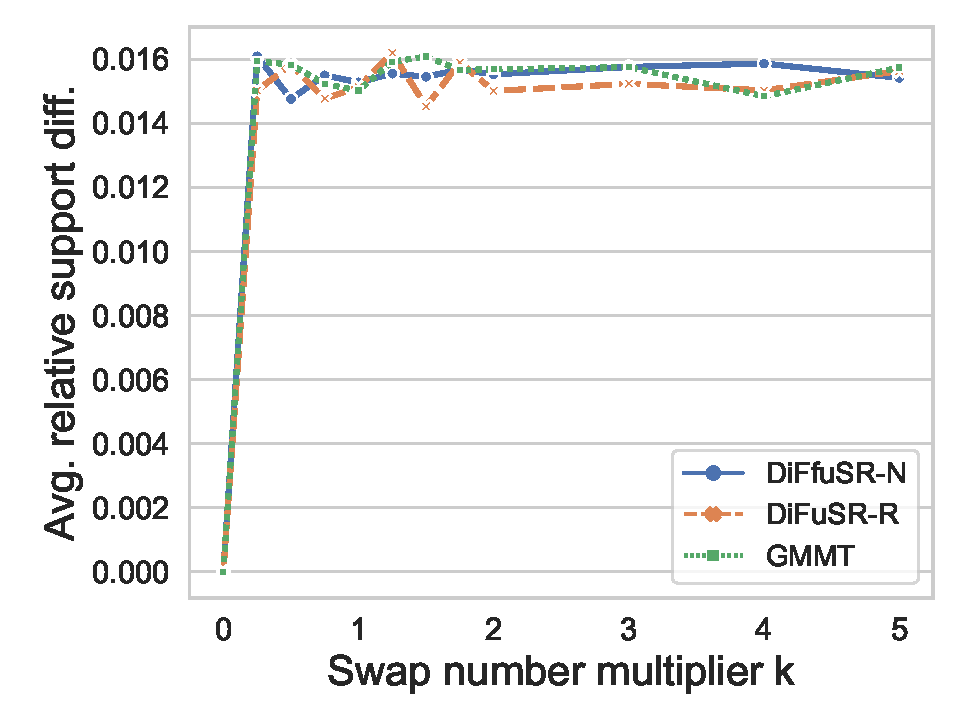
\includegraphics[width=\textwidth]{convergence-chess-5-0.8-0.pdf} % chktex 8
      \caption{\textsc{Chess}}
    \end{subfigure}%
    \begin{subfigure}{0.33\textwidth}
      \centering
      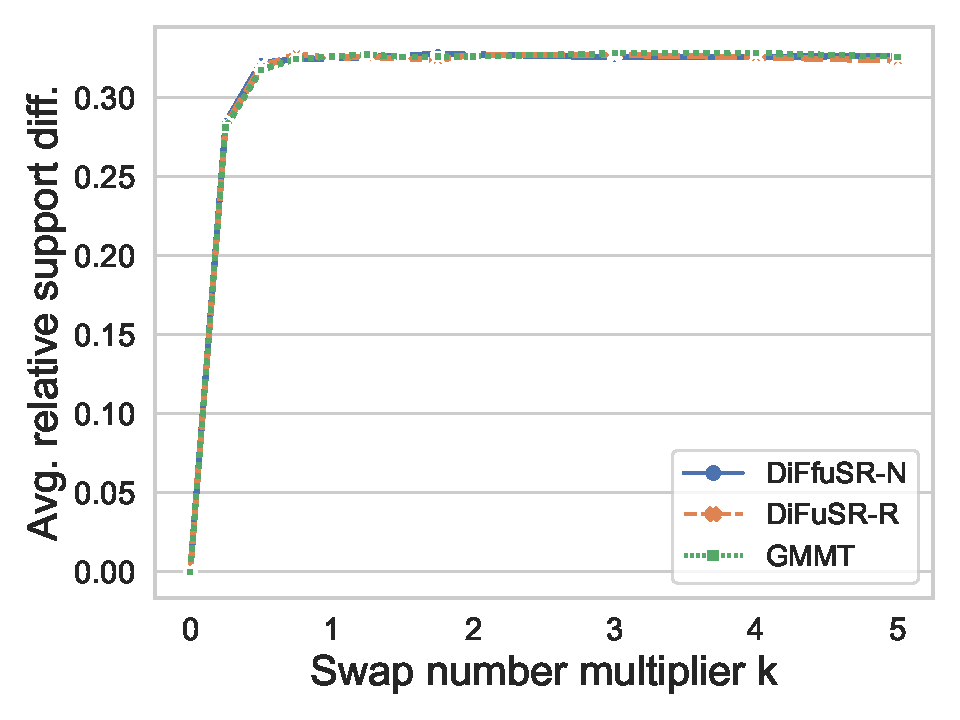
\includegraphics[width=\textwidth]{convergence-mushrooms-5-0.3-0.pdf} % chktex 8
      \caption{\textsc{Mushroom}}
    \end{subfigure}%
    \begin{subfigure}{0.33\textwidth}
      \centering
      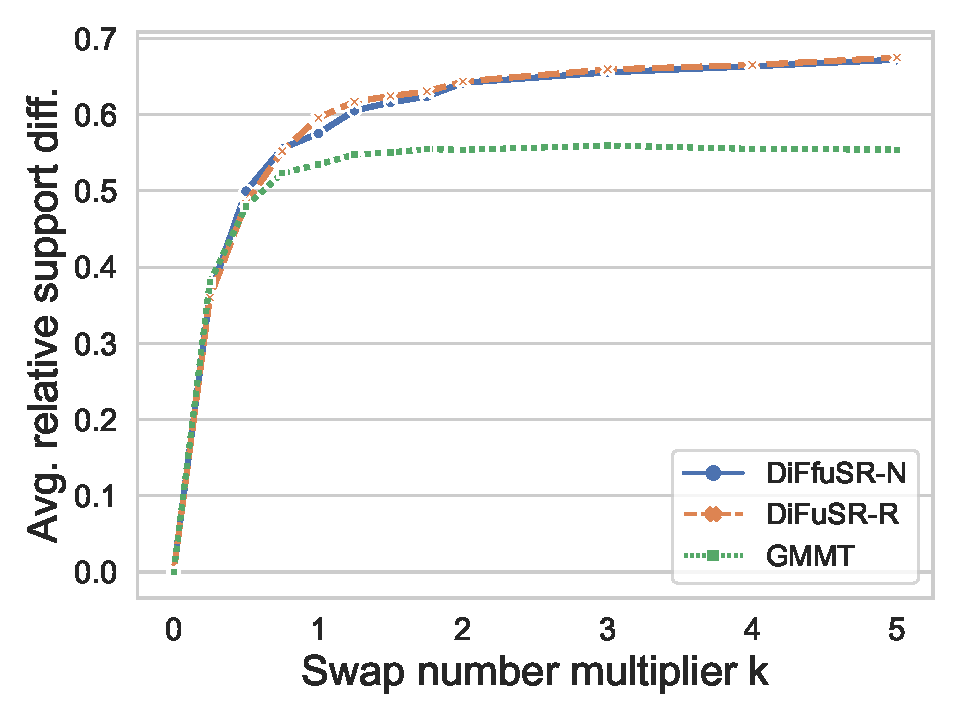
\includegraphics[width=\textwidth]{convergence-BMS1-5-0.001-0.pdf} % chktex 8
      \caption{\textsc{BMS 1}}
    \end{subfigure}
  \end{figure}
  \begin{itemize}
    \item All methods need $2 \sumtlen$ swaps, where $\sumtlen \doteq \sum_{i =
      1}^{m} \card{t_i}$, which is \emph{pretty fast}.
    \item Possible \emph{future direction}: prove an \emph{upper bound} to the
      mixing time.
  \end{itemize}
\end{frame}

\begin{frame}{Conclusion}
  \begin{itemize}
    \item \emph{Sampling datasets} from the null model is a key step in
      evaluating the statistical validity of observed results.
    \item Want: \emph{statistically correct} and \emph{computationally
      efficient} methods to sample datasets.
    \item Issue: existing method samples datasets from the null model \emph{with}
      distortion.
    \item Solution: our methods sample datasets from the null model
      \emph{without} distortion.
  \end{itemize}
\end{frame}

\end{document}
